\documentclass[11pt,a4j]{jarticle}
\usepackage{ascmac}
\usepackage{times}
\usepackage{graphicx}

\setlength\textwidth{17.0cm}
\setlength\textheight{26.0cm}

%ページ上の余白
\setlength\topmargin{-2.54cm}

%奇数ページ左の余白
\setlength\oddsidemargin{-0.54cm}

%偶数ページ左の余白
\setlength\evensidemargin{-0.54cm}

\begin{document}
\noindent
\begin{flushright}
{\small	2007.01.08}
\end{flushright}
\begin{center}
{\large\bf PENクイックリファレンス}
\end{center}

\begin{enumerate} \itemsep 0pt  \parskip 0pt
\item 基本画面 \\
\begin{figure}[htbp]
  \begin{center}
    \vspace{-0.5cm}
    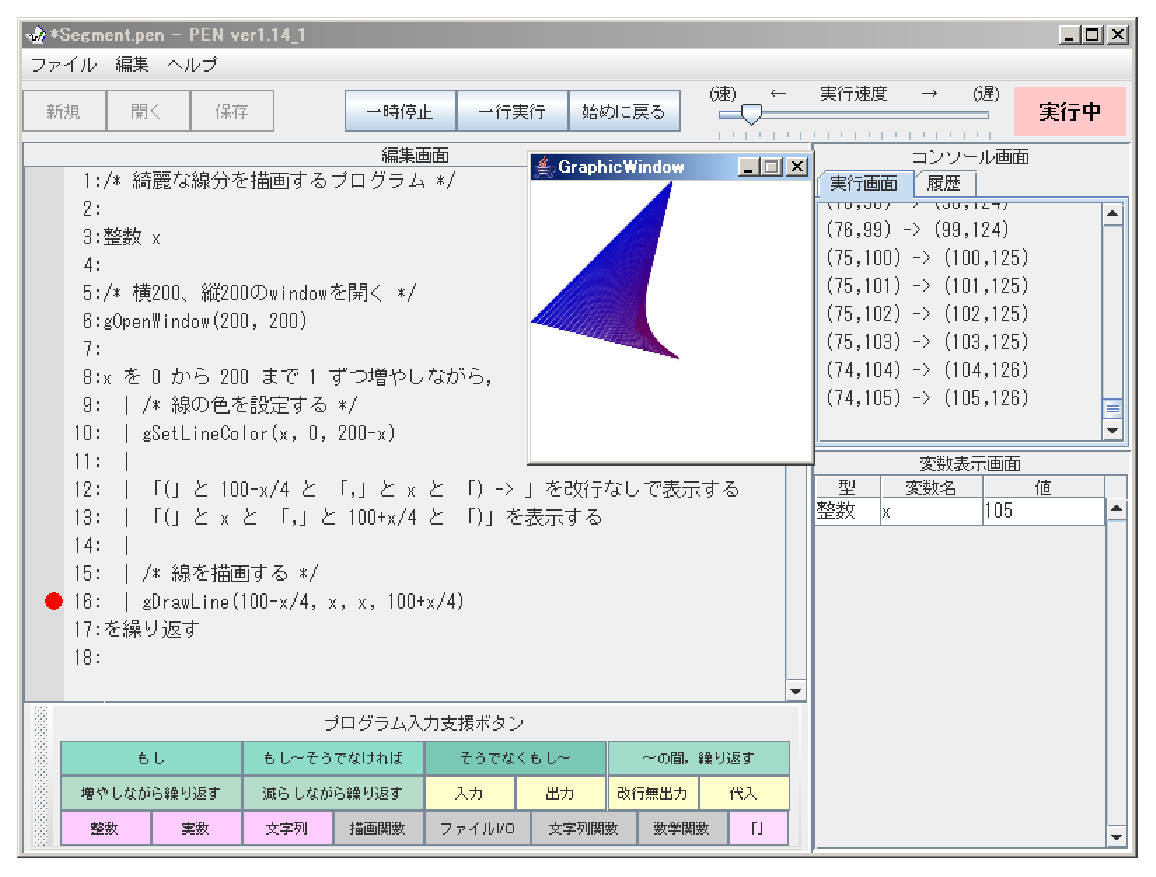
\includegraphics[width=12.0cm]{./eps/pen001.eps}
    \vspace{-1.0cm}
  \end{center}
\end{figure}
  
\begin{enumerate} \itemsep 0pt  \parskip 0pt
\item 編集画面 \\
プログラムのソースコードを入力するエリアです。 

\vspace{0.2cm}

\item コンソール画面 \\
プログラム中の出力はこの画面に表示されます。
また、入力もこの画面から行います。 \\
タブの操作により表示方法の異なる「実行画面」と「履歴」に切り替えられます。 
\begin{itemize} \itemsep 0pt  \parskip 0pt
\item 実行画面 : 実行中もしくは実行直後のコンソールが表示されます。
\item 履歴     : 今までの実行した結果の全てが表示されます。
\end{itemize}

\vspace{0.2cm}

\item 変数表示画面 \\
データ型、変数名と、変数に代入されている値が表示されます。 \\
プログラム実行時に変数の値の変化を観察することができます。 

\vspace{0.2cm}

\item プログラム入力支援ボタン \\
プログラムの入力を補助するためのボタンです。 \\
\begin{minipage}{12.0cm} \begin{itembox}[l]{「もし〜そうでなければ」のボタンで入力されるコード} \begin{verbatim}
もし ≪条件式≫ ならば
  |
を実行し,そうでなければ
  |
を実行する
\end{verbatim} \end{itembox} \end{minipage} \\
≪条件式≫など≪≫に囲まれた部分にカーソルを移動すると≪≫の部分全体が選択され、 \\
そこに書くべき式などに簡単に書き換えることができます。

\vspace{0.2cm}

\item GraphicWindow \\
図形描画の出力はこのウィンドウに表示されます。 \\
描画関連の命令は `xDNCL-Draw.pdf' をご覧ください。
\end{enumerate}

\newpage

\item 実行時の画面 
\begin{figure}[htbp]
  \vspace{-0.3cm}
  \begin{center}
    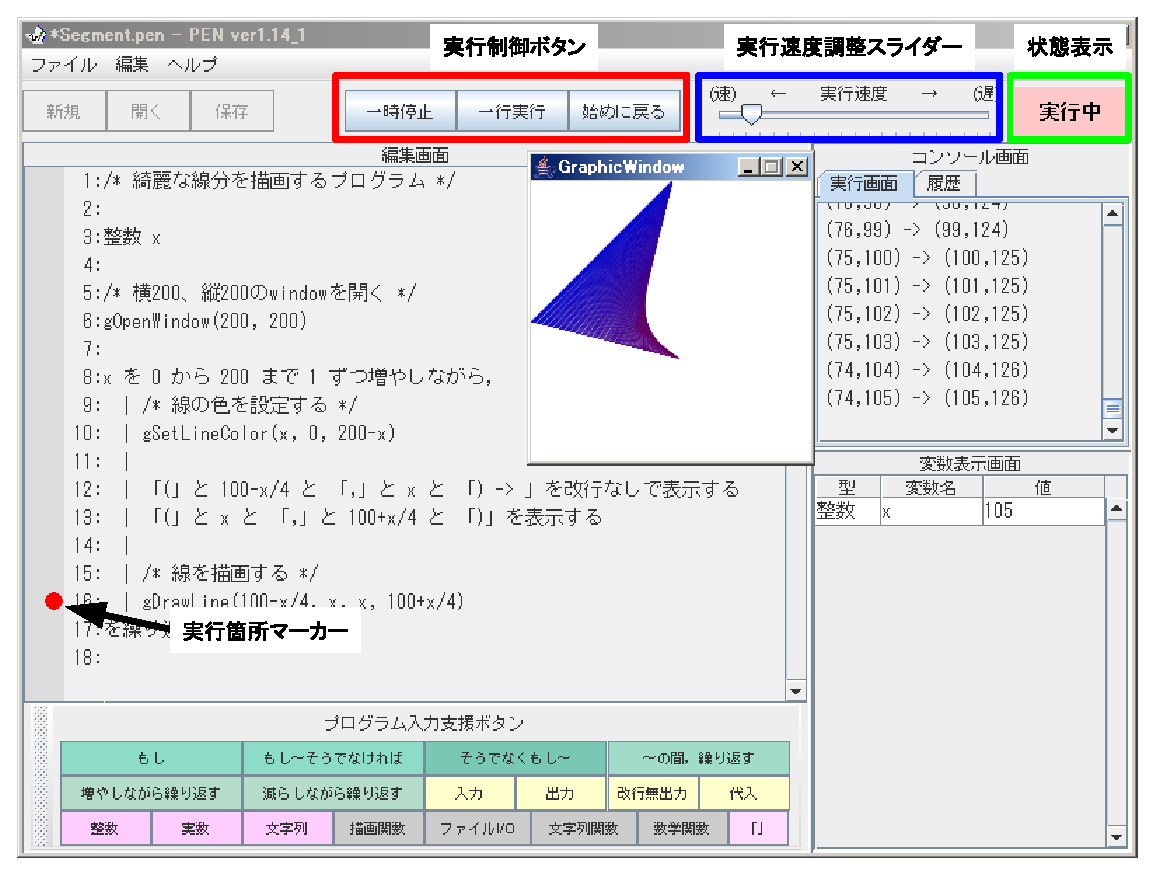
\includegraphics[width=12.0cm]{./eps/pen002.eps}
    \vspace{-1.0cm}
  \end{center}
\end{figure}

\begin{enumerate} \itemsep 0pt  \parskip 0pt
\item 実行制御ボタン
\begin{table}[htbp]
  \vspace{-0.3cm}
  \begin{center}
    \begin{tabular}{l|p{11.0cm}} \hline
	状態表		& 意味 \\ \hline
	実行		&
                  プログラムを実行する場合はこのボタンを押します。
                  プログラム実行中は「一時停止」ボタンに変化します。
                  実行する速度は「実行速度調整スライダー」で変化させることができます。 \\ \hline
    始めから実行&
                  実行ボタンと同じ。 \\ \hline
    一時停止	&
                  プログラム実行中に押すと実行を一時停止することができます。
                  一時停止時は、「再開」のボタンに変化します。 \\ \hline
    再開		&
                  一時停止状態から実行を再開したい場合に使用します。
                  再開後は、「一時停止」のボタンに変化します。 \\ \hline
	一行実行	&
	              「実行箇所マーカー」のある行を実行し、その後、一時停止状態になります。 \\ \hline
	始めに戻る	&
	              プログラムの実行を取り止め、プログラムの最初に戻ります。 \\ \hline
    \end{tabular}
  \end{center}
  \vspace{-0.7cm}
\end{table}

\vspace{0.2cm}

\item 実行速度調整スライダー \\
プログラムの実行速度を変更するためのスライダーです。 \\
バーをゲージの左側に移動すると実行速度が速くなり、右側に移動すると遅くなります。

\vspace{0.2cm}

\item 状態表示
\begin{table}[htbp]
  \vspace{-0.3cm}
  \begin{center}
    \begin{tabular}{l|p{11.0cm}} \hline
	状態表		& 意味 \\ \hline
	実行待ち	& プログラムを実行していない状態。
				プログラムの編集が可能。 \\ \hline
	実行中		& 通常にプログラムを実行している状態。 \\ \hline
	一時停止中	& 「一時停止」や「一行実行」によって実行
			  	が停止されている状態。 \\ \hline
	入力待ち	& プログラム内の入力文による入力待ち状態。
				入力はコンソール画面に行う。 \\ \hline
	実行終了	& プログラムの実行が終了した状態。
			 	再度、プログラムを実行する場合は
				「始めから実行」で行う。
				また状態を「実行待ち」に初期化する
				には「始めに戻る」で行う。 \\ \hline
    \end{tabular}
  \end{center}
  \vspace{-0.7cm}
\end{table}

\vspace{0.2cm}

\item 実行箇所マーカー \\
これから実行する行を指し示しています。 \\
この場面では16行目を実行する直前の状態になります
\end{enumerate}
\end{enumerate}

\end{document} 
